\chapter{Semantic Analysis (SA)}
The semantic analysis phase checks the source programs for semantic errors and gathers type information for the subsequent code-generation phase.
\begin{description}
    \item[Type Checks]\mbox{} \\
    The type of a construct must match that expected by its context;
    \item[Name-Related and Uniqueness Checks]\mbox{} \\
    Objects must be declared once;
    \item[Flow-of-Control Checks]\mbox{} \\
    Statements (such as \emph{break} and \emph{continue}) that cause flow of control to leave a construct must have a place where to go.
\end{description}

\section{Type Expressions}
A type expression $T$ denotes the type of a language construct, that can be:
\begin{itemize}
    \item a basic type;
    \item a type construct applied to type expressions.
\end{itemize}
The expressions can be conveniently represented by trees or DAGs with:
\begin{itemize}
    \item type constructors as interior nodes;
    \item basic types or type names as leaves.
\end{itemize}

\chapter{Intermediate-Code Generation (ICG)}
\section{Intermediate Representations}
\subsubsection{Syntax Tree}
Condensed from a parse tree where operators and keywords replace their non-terminal parent nodes.
\begin{figure}[H]
    \centerline{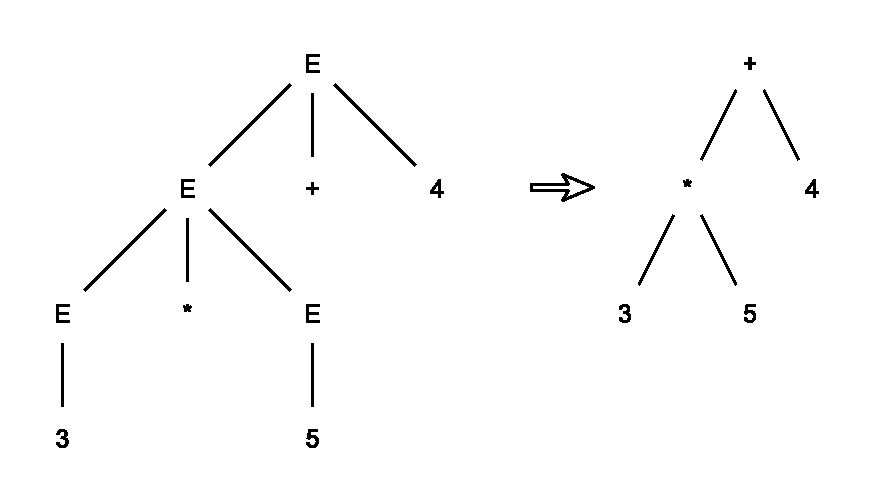
\includegraphics[width=0.6\textwidth]{img/15.pdf}}
\end{figure}

\subsubsection{Three-Address Code}
Linearised representation of a syntax tree in which explicit names correspond to interior node.
$$
    a = b \ast -c + b \ast -c
$$
\begin{figure}[H]
    \centerline{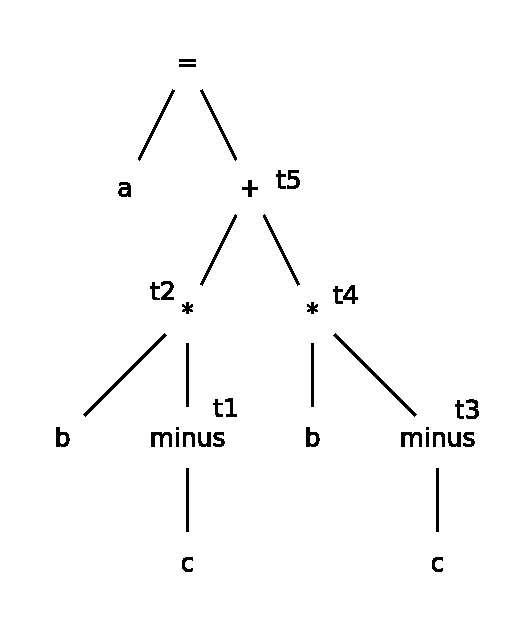
\includegraphics[width=0.4\textwidth]{img/16.pdf}}
\end{figure}
\begin{align*}
    t_1 &= minus c \\
    t_2 &= b \ast t_1 \\
    t_3 &= minus c \\
    t_4 &= b \ast t_3 \\
    t_5 &= t_2 + t_4 \\
    a &= t_5
\end{align*}

\section{Scope of Declaration}
\subsubsection{Scope of a Declaration of an Identifier $X$}
The region of program in which uses of $X$ refer to this declaration.
\subsubsection{Static (lexical) Scope}
The scope of a declaration is determined by where the declaration appears in the program and by keywords like public, private, and protected.
\subsubsection{Multiple Declaration}
Nested environments are allowed, where identifiers can be redeclared.
\subsubsection{Most-Closely Nested Rule}
An identifier $X$ is in the scope of the most-closely nested declaration of $X$.

\section{Symbol Tables}
Symbol tables are data structures used to hold information about source-program constructs.
Information is collected incrementally in the analysis phase and used in the synthesis phase to generate the code.
Entries in the symbol table contain information about an identifier (character string, type, position, \ldots).
Multiple declarations of the same identifier can be supported by setting up a separate symbol table for each scope.
The most-closely nested rule can be implemented by chaining the symbol tables (the table for a nested scope points to the table for its enclosing scope).

\section{Storage Layout for Sequence of Declarations}
Example:
\begin{align*}
    P &\to \left\{offset = 0\right\}D \\
    D &\to D_1D_2 \\
    D &\to T_{id}; \left\{top.put(id.lexeme, T.type, offset); \right. \\
        &\qquad \left. offset = offset + T.width\right\}
\end{align*}
Variable $offset$ keeps track of the next available relative address.
Function $top.put(id.lexeme, T.type, offset)$ creates a symbol-table entry for $id.lexeme$, with type $T.type$ and relative address $offset$ in the data area of the current $(top)$ symbol table.

\section{Storage for Records}
The production $T \to record\left\{D\right\}$ adds record types since field name $X$ in a record type does not conflict with other uses of $X$, each record type will get its own symbol table.
The offset for a field name is relative to the data area of its symbol table.
A record type can be represented by the type expression $record(t)$, where $t$ is a symbol table that holds information about the fields of the record.
Example:
\begin{align*}
    T &\to record\left\{\left\{Env.push(top); top = new Env(top); \right.\right. \\
            &\qquad \qquad \left.\left. Storage.push(offset); offset = 0\right\} \right. \\
        &\qquad \left. D\right\} \left\{T.type = record(top); T.width = offset; \right. \\
            &\qquad \qquad \left. top = Env.pop(); offset = Storage.pop()\right\}
\end{align*}
Functions $Env.push(top)$ and $Storage.push(offset)$ save the current symbol table and offset onto stacks.
Functions $Env.pop()$ and $Storage.pop()$ retrieve the saved symbol table and offset.

\section{Translation of Assignment Statements}
Example:
\begin{align*}
    S &\to id = E; \left\{gen(top.get(id.lexeme) = E.addr)\right\} \\
    E &\to E_1 + E_2 \left\{E.addr = new Temp(); gen(R.addr ``='' E_1.addr ``+'' E_2.addr)\right\} \\
    &\qquad| -E_1 \left\{E.addr = new Temp(); gen(E.addr ``='' ``minus'' E.1_addr)\right\} \\
    &\qquad| (E_1) \left\{E.addr = E_1.addr\right\} \\
    &\qquad| id \left\{E.addr = top.get(id.lexeme)\right\}
\end{align*}
Function $gen(three-address instruction)$ constructs a three-address instruction and appends it to the sequence generated so far.
Function $top.gen(id.lexeme)$ retrieve the entry for $id.lexeme$ in the data area of the current $(top)$ symbol table.

\section{Translation of Boolean Expression}
$AND(\&\&)$ and $OR(||)$ operators are left associative; $NOT(!)$ takes precedence over $AND$, which takes precedence over $OR$.

\section{Back-Patching}
Function $makelist(i)$ creates a new list of jumps containing only the index $i$ into the sequence of instructions (returns a pointer to the newly created list).
Function $merge(p_1, p_2)$ concatenates the lists pointed to by $p_1$ and $p_2$ (returns a pointer to the concatenated list).
Function $backpatch(p, i)$ inserts $i$ as the target label for each of the instructions on the list pointed to by $p$.